\section{Results}
\label{sec:results}

\subsection{Functional evaluation exposes different weaknesses}
\label{sec:baseline_results}
% Generated from frozen audited summaries by build_paper_figures.py.
\begin{table*}[t]
\centering
\small
\setlength{\tabcolsep}{5.5pt}
\caption{Complete v5 results for seven baseline configurations and two CF-MoA instantiations. Scores are percentages of native-unit means; bold denotes the highest value in each column.}
\label{tab:main-system-results}
\begin{tabular}{llrrrrrr}
\toprule
System & Backbone & ALL & R1 & R2 & R3 & R4 & R5 \\
\multicolumn{2}{l}{\emph{Comparison units}} & 6,104 & 2,866 & 79 & 733 & 13 & 3,600 \\
\midrule
Direct & Llama & 48.10 & 30.04 & 8.86 & 17.87 & 38.46 & 65.70 \\
MedRGAG & Llama & 48.81 & 31.33 & 7.59 & 24.69 & 53.85 & 65.88 \\
MA-RAG & Qwen & 51.61 & 26.73 & 34.18 & 8.59 & 38.46 & \textbf{73.37} \\
MedRAG & Llama & 48.20 & 27.84 & 29.11 & 30.42 & 53.85 & 65.28 \\
MedRAG & Qwen & 47.35 & 28.58 & 41.77 & 25.24 & 53.85 & 63.42 \\
MedGENIE & Llama & 48.02 & 29.94 & 18.99 & 21.42 & \textbf{61.54} & 65.15 \\
TC-RAG & Qwen & 49.43 & 31.44 & 29.11 & 28.92 & 30.77 & 66.17 \\
\midrule
\textbf{CF-MoA (B)} & Llama & 58.29 & 44.63 & 48.10 & 53.21 & 53.85 & 68.84 \\
\textbf{CF-MoA (B)} & Qwen & \textbf{59.36} & \textbf{46.62} & \textbf{58.23} & \textbf{60.03} & 23.08 & 68.79 \\
\bottomrule
\end{tabular}
\par\smallskip
\begin{minipage}{0.97\textwidth}\footnotesize Each configuration covers 13,905 unique inputs. ALL averages non-reference task scores within units and then across units; R labels may overlap. Llama denotes Llama-3.1-8B-Instruct and Qwen denotes Qwen3-8B. The selected MedRAG-Llama baseline includes its output repair.\end{minipage}
\end{table*}


The seven baselines occupy a narrow range on the aggregate metric but exhibit substantially different functional profiles (Table~\ref{tab:main-system-results}). MA-RAG has the highest baseline aggregate score, 51.61, and the highest preservation score, 73.37, yet scores 8.59 on candidate comparison. \sysQ{} leads the baselines on support removal at 41.77, while \sysL{} leads on candidate comparison at 30.42. Direct answering reaches 48.10 overall but only 8.86 on support removal. Thus, a system can answer many ordinary or preservation-oriented items correctly while struggling to revise the support for a specific decision.

The taxonomy makes these differences actionable. Support removal calls for checking whether an answer's prerequisites still hold; diagnosis calls for comparing viable candidates under the changed evidence. Neither need is fully described by the number of retrieved passages or generated answers. This distinction motivates the specialized operations evaluated next.

\subsection{Specialized heads transfer across seven configurations}
\label{sec:head_results}
\begin{figure*}[t]
\centering
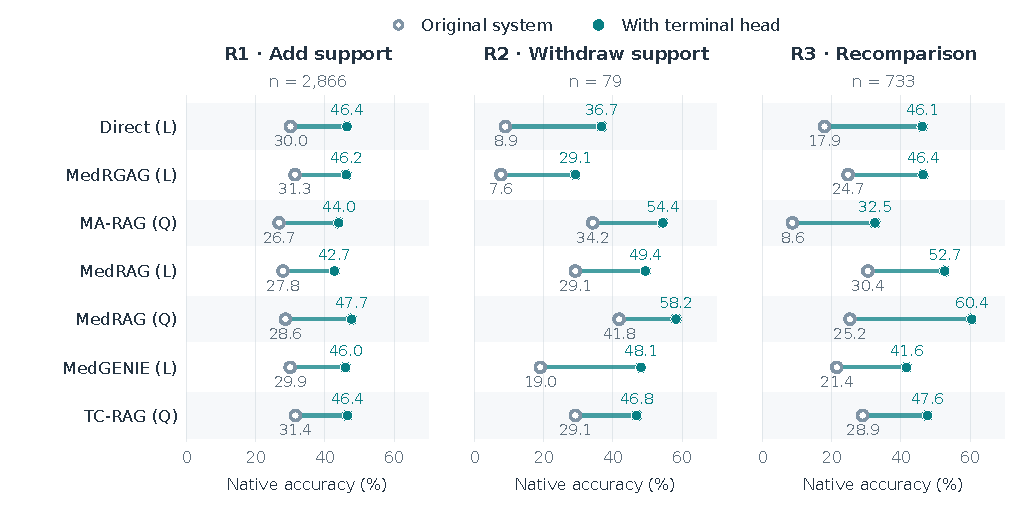
\includegraphics[width=\textwidth]{seven_system_head_gains.pdf}
\caption{Original and head-augmented performance across all seven configurations. Each panel uses the complete corresponding category: support addition ($n=2{,}866$), support removal ($n=79$), and candidate comparison ($n=733$). All 21 comparisons improve. Category memberships overlap; exact correct counts and branch coverage are in Appendix~\ref{app:heads}.}
\label{fig:seven-head-gains}
\end{figure*}

Figure~\ref{fig:seven-head-gains} shows improvements in all 21 system--category comparisons. Support addition rises from an original range of 26.73--31.44\% to 42.74--47.70\%; support removal rises from 7.59--41.77\% to 29.11--58.23\%; and candidate comparison rises from 8.59--30.42\% to 32.47--60.44\%. The gains occur across direct answering, retrieval-based systems, and systems with their own agent or control loops. They show that a functional head can repair failures left by different upstream workflows.

The head construction reflects the overlap between categories. On support addition, the adopted wrapper routes 1,780 units to diagnosis, 72 to rule execution, and retains the original result on 1,014 units. On candidate comparison, 680 units use diagnosis, ten use rules, and 43 retain their original result. These shared operations connect the category analysis to an implementable system, while avoiding a separate learned model for every label.

\paragraph{Candidate presentation accounts for much of the diagnosis gain.}
On the 680-unit diagnostic subset, averaging across the seven systems, the original score is 20.97\%, a single catalog decision reaches 45.44\%, six uncalibrated decisions reach 46.47\%, and calibrated decisions reach 46.13\%. The largest common improvement therefore comes from asking the model to make an explicit decision over the available diagnoses. Additional voting and calibration have smaller, configuration-dependent effects. For \sysL{}, the correct count changes from 203 to 339 with one catalog decision and to 359 with either six-decision variant. For \sysQ{}, the corresponding counts are 160, 382, 402, and 410. Appendix~\ref{app:heads} gives every configuration and additional source checks.

\paragraph{Both support operations contribute.}
% Generated from frozen audited summaries by build_paper_figures.py.
\begin{table}[t]
\centering
\small
\setlength{\tabcolsep}{6pt}
\caption{Support-operation ablation on all 123 rule inputs, reusing the same extracted facts and execution states. Parentheses give the change in correct outputs relative to the complete kernel.}
\label{tab:support-ablation}
\begin{tabular}{lrr}
\toprule
Policy & Llama & Qwen \\
\midrule
Full support kernel & 69/123 & 71/123 \\
Without add & 43/123 (-26) & 48/123 (-23) \\
Without remove & 53/123 (-16) & 60/123 (-11) \\
\bottomrule
\end{tabular}
\par\smallskip
\begin{minipage}{\linewidth}\footnotesize A1 and A2 share one rule kernel. Unavailable outputs remain in the denominator.\end{minipage}
\end{table}

The shared support executor uses the extracted facts to add newly justified options and remove contradicted ones. On the 123-input control in Table~\ref{tab:support-ablation}, disabling addition reduces correct answers from 69 to 43 for Llama and from 71 to 48 for Qwen. Disabling removal reduces them to 53 and 60. Both operations contribute under the same fact extraction and rule statuses.

The small support-removal category also exposes a dataset prior: a coverage-matched constant ``None'' control obtains more correct answers than the head in each of the seven configurations. The head's value is therefore better assessed together with the operation ablation and the nine covered prescribing examples with remaining support, where the constant control scores zero. On these nine examples, five configurations improve, one is unchanged, and one declines. This result favors explicit support execution as a useful operation while showing why the raw category average alone is an incomplete diagnosis.

\subsection{The complete controller improves overall and paired correctness}
\label{sec:full_results}

On the complete benchmark, the aggregate score rises from 48.20 to 58.29 for \sysL{} and from 47.35 to 59.36 for \sysQ{} (Table~\ref{tab:main-system-results}). The gains are 10.09 percentage points (95\% family bootstrap interval: 8.96--11.23) and 12.01 points (10.92--13.15). Both configurations improve on support addition, support removal, candidate comparison, and preservation. Their final scores also exceed the highest aggregate baseline, although the within-configuration contrasts provide the direct measure of the controller's effect.

On the 13 clinical consequence units, \sysL{} remains at 53.85 while \sysQ{} decreases from 53.85 to 23.08 under the readout branch. This localized regression is retained in the main table alongside the larger-category gains.

\begin{figure*}[t]
\centering
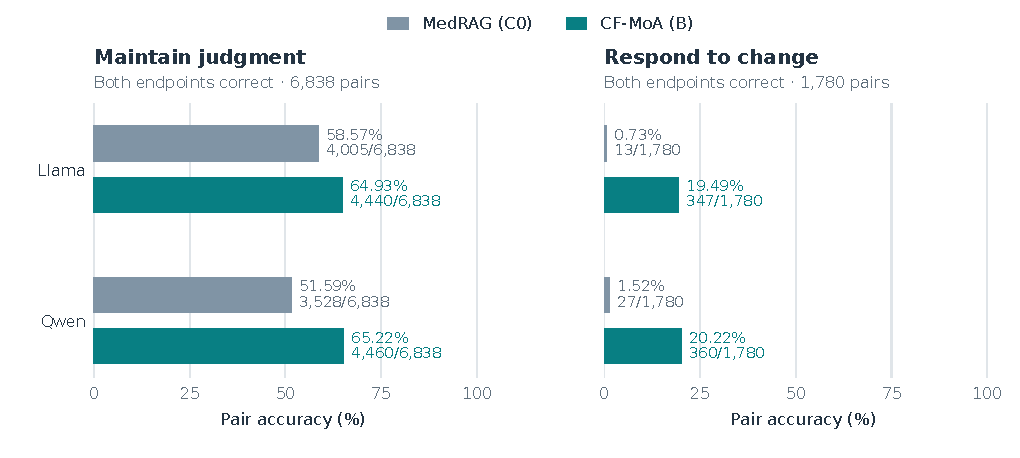
\includegraphics[width=\textwidth]{paired_behavior.pdf}
\caption{Correctness on both members of a pair. On answer-preserving pairs, correct counts increase from 4,005 to 4,440 for Llama and from 3,528 to 4,460 for Qwen ($n=6{,}838$). On answer-changing pairs, they increase from 13 to 347 and from 27 to 360 ($n=1{,}780$). Agreement alone does not satisfy either measure.}
\label{fig:paired-behavior}
\end{figure*}

Paired evaluation tests the behavior that motivates the benchmark (Figure~\ref{fig:paired-behavior}). On answer-preserving pairs, both-side correctness rises from 58.57 to 64.93\% for Llama and from 51.59 to 65.22\% for Qwen. On answer-changing pairs, it rises from 0.73 to 19.49\% and from 1.52 to 20.22\%, respectively. All four paired differences have positive family-bootstrap intervals. The controller thus improves selective response to a change as well as correctness under a change that should leave the answer intact. The lower absolute scores on changing pairs identify evidence-sensitive updating as a continuing challenge.

\subsection{Conditional execution and stable readout}
\label{sec:conditional}

The consequence agent addresses tasks with an explicit executable model. On 24 virtual physiological profiles with 12 questions each, typed local intervention produces correct binary and numerical outputs on all 288 questions for both backbones. A same-tools alternative that asks the model to generate a complete plan obtains 270 and 222 correct numerical outputs. Removing the intervention from the patch procedure reduces numerical correctness to 67 for both backbones. These controls support the value of a constrained local edit followed by execution in the supplied model (Appendix~\ref{app:model}).

Stable readout is evaluated on a separate 208-group component panel combining answer sampling and NLI interfaces. Its group-weighted paired score improves from 60.19 to 65.90\% for Llama and from 59.17 to 66.47\% for Qwen. In the final 16-group extension, both-side correctness improves from 11 to 12 groups and from 12 to 13 groups relative to the matched single-answer control. These observations motivated its use as the broad readout branch of the adopted controller.

\subsection{More aggregation is not uniformly better}
\label{sec:extensions}

We evaluated further aggregation on the same full input set. A rationale-conditioned verifier scores the distinct candidates already present in the saved readout pool and returns an existing complete answer. Relative to B, it changes the aggregate score by $-1.81$ points for Llama and $+0.93$ points for Qwen. Its candidate-only and joint-selection counterparts likewise do not provide a consistent improvement over B; three additional sampled answers yield 58.32 and 59.67, with more unavailable outputs. The complete six-arm comparison is retained in Appendix~\ref{app:full}. Earlier generated-answer aggregation also underperformed the adopted controller on its development panel. These results support sparse execution of useful operations as the default \cfmoa{} design.

The controller adds measurable computation. Attributed component requests total 59,800 for Llama and 58,301 for Qwen, before the original answering and retrieval costs. Rationale-conditioned verification adds 13,308 and 9,820 requests. This cost and its mixed gains make it a less attractive default than the adopted controller; Appendix~\ref{app:cost} gives the physical request and token accounting.
